% первая часть

\section{Анализ предметной области}
\subsection{Принципы Умного города}
Термин Умный город появился относительно недавно, и определенного конкретного определения этому понятию нет. Но, все-таки  эксперты сошлись в том, что главный источник управления <<смарт сити>> --- данные о населении.

Умный город (smart city) --- это стратегическая концепция по развитию городского пространства, подразумевающая совместное использование информационно - коммуникационных технологий (ИКТ) и решений Интернета вещей (IoT) для управления городской инфраструктурой. К нему относятся транспортные системы, водопроводные каналы, медицинские организации, системы переработки отходов и множество других общественных служб. \cite{Harrison} 

Главная идея системы Умный город --- организация информационного пространства, которое содержит в себе данные о работе контролируемых объектов (счетчиков тепловой и электрической энергии, лифтов, электротехнического оборудования, различных технических средств безопасности и т.д.). На любом расстоянии можно управлять объектами в режиме реального времени, вне зависимости от места расположения объектов и центрального управляющего пункта в городе.\cite{NK}

Найти слабые места в работе организации, поставщиков ресурсов, оборудования и персонала, а так же можно проанализировать данные. Введение в эксплуатацию системы Умный город позволяет не только контролировать работу оборудования, но и принимать максимально верные управленческие решения. 

Для целостной системы Умный город должны быть функционально законченные подсистемы:
\begin{itemize}
	\item диспетчеризации и контроля лифтов; 
	\item автоматизированного коммерческого контроля и учета энергоресурсов и электроэнергии; 
	\item охранно-пожарной сигнализации и видеонаблюдения; 
	\item контроля доступа к помещению и к оборудованию; 
	\item управления оборудованием и инженерными сооружениями; 
	\item другие дополнительные системы, такие как контроль затопления подвалов, сигнализация загазованности горючими газами, экстренной голосовой связи.
\end{itemize}

Основные принципы Умного города: 
\begin{itemize}
	\item микрорайон как градостроительная единица; 
	\item автономность города социальная, деловая и  культурная самодостаточность;
	\item разработка по стандартам экологичного строительства; 
	\item использование новейших информационных и коммуникационных технологий;
	\item внедрение инновационных технологий энергетики, транспорта и строительства;
\end{itemize}

Основными механизмами правильной организации и  оптимизации использования ресурсов в Умном городе являются: 
\begin{itemize}
	\item снижение неравномерности потребления в период пиков и провалов (основная проблема всех инфраструктур), т.е. распределение нагрузки на инфраструктурные сети во времени; 
	\item создание сетевых, а не линейных систем поставки ресурса позволят маневрировать потоками и «обходить» аварийные или пиковые участки, т.е. распределение в пространстве; 
	\item создание динамически управляемых источников мощности: накопители, демпферы, малоинерционные генераторы и др.; 
	\item создание распределенной генерации различного масштаба;
	\item снижение потерь и ресурсопотребления конечных пользователей (Умные дома, энергоэффективное оборудование и др.).
\end{itemize}

\subsection{Актуальные проблемы Умных городов}
Рассматривая возможные негативные аспекты Умных городов, надо иметь в виду несколько нюансов.\cite{Almanah} Конечно же, проблема приватности к ним относится. Мы даже не осознаем, насколько огромные объемы данных о нас постоянно создаются и сохраняются. Google знаком с нашими поисковыми привычками в интернете, с нашим отношением к покупкам, с нашей персональной информацией и т.д. Камеры по всему городу отслеживают перемещения людей и машин, высматривают угрозы безопасности, происшествия и прочие аномалии. Участвовать или не участвовать в наиболее персональных аспектах Умных городов и сборе информации о людях должно быть личным делом каждого. Также должны существовать надежные способы шифрования и последующего уничтожения информации об индивидах, чтобы гарантировать их право на личную жизнь.

Инвестиции в Умные города и расходы на их методы функционирования и технологии высоки на начальном этапе, но с течением времени эти расходы превращаются в долгосрочную экономию. Это означает, что политики, избранные всего на несколько лет, вполне могут не быть заинтересованы в инвестициях в долгосрочные стратегии. Поэтому должен существовать консенсус между политиками и их электоратом относительно того, в каком направлении движется развитие города, каковы его приоритеты и во что нужно инвестировать.

Координация — вот еще один важный аспект для внедрения передовых практик в Умный город. Чтобы городские службы были эффективны, их необходимо координировать. Зачастую технологии или различные услуги предоставляются разными компаниями. Эти компании должны понимать, что в их интересах и в интересах жителей города работать вместе, а не просто продавать как можно больше товаров или услуг. Городские управленцы должны понимать концепцию Умного города и делать так, чтобы скоординированные инвестиции направлялись на достижение наилучшего желаемого результата.

\subsection{Пример Умного города}
В штате Колорадо есть город Боулдер население которого около 100 тыс. человек. Этот город стал первым Умным городом в мире. Жители этого замечательного города сразу же приобрели репутацию «хранителей» окружающей среды. Они применяют новейшие технологии, которые намного меньше вредны для нашей природы. Дома жителей Боулдера наполнены самыми последними экологичными и энергосберегающими устройствами: панелями солнечных батарей, электрическими автомобилями и специализированными системами обогрева, охлаждения и освещения, которые объединяются единой системой мониторинга, сообщающей домовладельцу данные об углеродном следе дома (то есть количество CO2, поступающего в атмосферу). Рей Гогель из Xcel Energy, член сервисной компании, которая внедрила новую систему, сказал: «Нам нравится думать об Умной электросети как о примирении мира Томаса Эдисона с миром Билла Гейтса. Мы делаем то, в чем нуждаются все». В этом городе определенные дома имеют возможность самостоятельно управлять энергосберегающими технологиями. 

Очень актуальными являются солнечные батареи и интеллектуальные счетчики. Контролировать потребление энергии достаточно легко благодаря новой системе. Управление автомобилем, гаражом, домом можно осуществлять через компьютер. Все части дома взаимосвязаны и общаются между собой. Все эти технологии очень экономичны и сильно упрощают жизнь людям. Есть такие горожане у которых счет за коммунальные услуги составляют всего 3 доллара в месяц. 

Очень удобной стала покупка автомобиля, можно выбрать его из списка по дате, цене или названию автосалона. Все можно сделать онлайн! Используя новую энергосистему можно решить, использовать возобновляемые источники или по-прежнему выбрать энергию сжигаемого угля. Для того, чтобы принять решение, не обязательно находиться в данном городе, достаточно выйти в Интернет, чтобы проследить за всеми процессами и управлять ими. Теперь не страшно оставить включенным какое-либо устройство, просто достаточно зайти через сеть и выключить. 

Такие многофункциональные системы --- это наше будущее. 

В скором времени интеллектуальные сети станут стандартом для всех новых домов. Каждый человек, конечно же, хочет минимально использовать энергию.

\subsection{Российские проекты Умных городов}
В России за последние годы появился ряд проектов по интеллектуализации городских сервисов. В основном это умное управление в трех сферах: электроэнергия, транспортные потоки, общественная безопасность.\cite{smartcity}
\subsubsection{ЦОД «Омский»}
Вокруг центра обработки данных «Омский» предполагается разместить промышленно-логистический парк (IT-кластер, высокотехнологичный сельскохозяйственный комплекс, производственные и лабораторные помещения), объекты жилой и социальной недвижимости (зона жилой застройки на 14 тыс. человек), административно-деловой центр и другие объекты. Технологии Умного города появятся в разработках самих резидентов кластера --- IT-компаний и стартапов в сфере облачных технологий. Подобно японским городам, «Омский» ставит целью перейти на самоокупаемость, энерго- и даже отчасти продуктовую независимость: например, самостоятельно генерировать электричество, а его избытки передавать на содержание теплиц.
\subsubsection{Ильинское-Усово}
Проектировщики ЖК «Ильинское-Усово» внедряют умные городские технологии уже на первой очереди строительства микрорайона: это новые материалы, Интернет вещей в части ЖКХ, безопасности и транспорта. ГК «Мортон» определяет 15 направлений развития Умного города, и отдает предпочтение решениям, которые охватывают сразу несколько из них. На фоне базовых технологий (интеграция транспортной и инженерной систем, энергосбережение, видеоаналитика и пр.) выделяется уникальная для России система недорогих решений в области медицины. Сама «Мортон» инвестирует в ряд городских технологий, которые впоследствии тиражирует.
\subsubsection{Владивосток}
Во Владивостоке работает Единая дежурная диспетчерская служба по управлению транспортом в реальном времени, а также автоматизированная система управления уличным освещением. «Ростелеком» внедряет в городе систему экстренного вызова оперативных служб и модернизированную систему оповещения.
\subsubsection{Белгород}
В Белгороде установлены Умное освещение и датчики на распределительных сетях, которые минимизируют последствия аварий.
\subsubsection{Екатеринбург}
Екатеринбург планирует создать интеллектуальную энергосеть к 2030 году. Столько займет модернизация существующих и построение новых энергообъектов с учетом требований Smart Grid, в том числе внедрение транспортных средств на электротяге, перевод объектов --- потребителей электроэнергии в режим ее генерации.

\subsection{Умный город в Обнинске}
В Обнинске в рамках федеральной программы <<Цифровая экономика РФ>> будет создан Умный город. Об этом было заявлено калужским губернатором Анатолием Артамоновым на инвестиционном форуме в Сочи в феврале 2018 года.

Выступая на сессии форума, калужский губернатор Анатолий Артамонов акцентировал внимание собравшихся, что для реализации данных проектов, необходимо, в первую очередь, совершенствовать инфраструктуру. Прежде всего, это касается городов, где она формировалась давно. По мнению губернатора, решение данной задачи возможно только при условии реализации единой госполитики. 

<<Это повлечет за собой большие расходы, но данное направление необходимо включить в число приоритетных>>, --- предложил Артамонов. Что касается Обнинска, то создание Умного города входит в стратегию социально-экономического развития наукограда на ближайшие 9 лет. 

<<Тема новая, но очень перспективная. Нам нужно стремиться к тому, чтобы в будущем не только крупные города, но и небольшие населенные пункты могли внедрить у себя Умные технологии>>, --- отметил губернатор. 

Ключевыми направлениями Умного города, охватывающими все виды социально --- экономической деятельности городов, являются: «Умная экономика», «Умная мобильность», «Умная среда», «Умные люди», «Умная безопасность», «Умная медицина», «Умное проживание» и «Умное управление». 

В целом, проект можно считать достаточно молодым. Находится он на стадии старта. Но уже успел завоевать доверие и признанность не в одной стране мира. Масштаб и продвижение проекта в разных точках мира зависят, в основном, от времени начала его ввода в пользование. 

Каждый житель города имеет право принимать участие в развитии проекта, предлагать идеи и проявлять интерес, к таким деталям, на которые, по его мнению, стоит обратить внимание. 

Умный город в Обнинске --- это информационный центр, обеспечивающий получение, обработку и предоставление информации по жизнеобеспечению и безопасности города. Организационная форма --- некоммерческое партнерство. Основой программы является понимание того факта, что все структуры, ответственные за комфортное и безопасное проживание в городе уже созданы. Задачей Программы является 
\begin{itemize}
	\item Повышение эффективности их деятельности путем применения новых технологий в области телекоммуникаций; 	
	\item Организация, в том числе, юридическая, более тесного взаимодействия предприятий; 
	\item Строительства и использования единой городской информационной структуры.
\end{itemize}

\subsection{Система «СТРИЖ»}
«СТРИЖ» — IoT-платформа на базе беспроводных LPWAN-сетей (Low-power Wide-area Network). Готовое решение для сбора данных в ЖКХ, промышленности, энергетике и других отраслях. \cite{strij}
\subsubsection{Описание системы}
Технология LPWAN (Low-power Wide-area Network) – беспроводная технология передачи небольших данных на большие расстояния рисунок~\ref{fig:lpwan}. 

\begin{figure}[H]
	\centering
	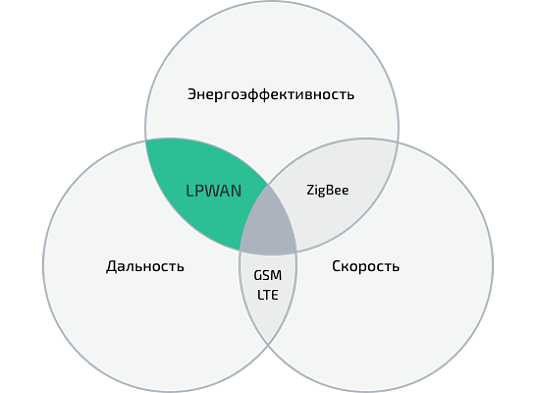
\includegraphics[width=0.7\linewidth]{pics/lpwan}
	\caption{Преимущества протоколов передачи данных}
	\label{fig:lpwan}
\end{figure}

В технологии LPWAN используется протокол XNB (Extended Narrowband). Он представляет собой переработку протокола связи на физическом уровне. XNB разработан для обмена данными устройств на больших распределенных территориях с минимальными затратами энергии рисунок~\ref{fig:strij}.

\begin{figure}[H]
	\centering
	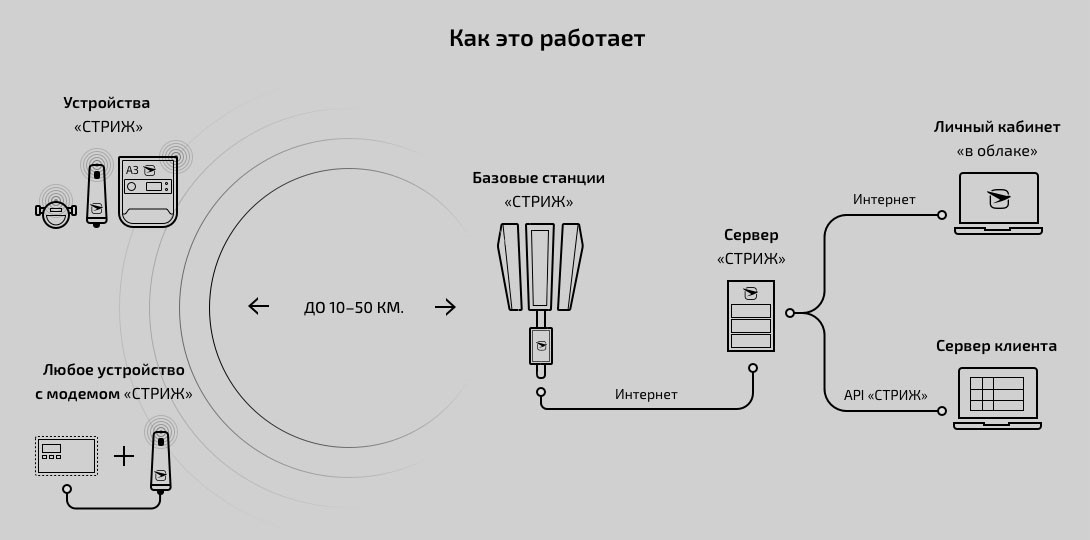
\includegraphics[width=0.7\linewidth]{pics/strij}
	\caption{Схема работы системы «СТРИЖ»}
	\label{fig:strij}
\end{figure}

Устройства и модемы «СТРИЖ» передают 8-байтные пакеты данных по беспроводному протоколу XNB на частоте 868,8 МГц (не требует лицензирования). Базовая станция принимает и обрабатывает сигналы от всех устройств «СТРИЖ» в радиусе 10—40 км.  Все станции передают данные на сервер. Сервер осуществляет обработку данных, мониторинг и управление устройств. Пользователь получает информацию в облачном личном кабинете «СТРИЖ» или по API в свое приложение.

\subsubsection{Достоинства и недостатки}

Система «СТРИЖ» обладает следующими преимуществами:

\begin{itemize}
	\item Передача данных до 50 км на открытой местности и до 10 км в городских условиях;
	\item Низкая энергозатратность, позволяет передавать данные по беспроводному каналу связи в течении нескольких лет, используя одну батарейку типа АА;
	\item Не нужно протягивать провода, позволяет устанавливать систему в уже построенные дома;
	\item Высокая проникающая способность благодаря технологии радиосвязи LPWAN;
	\item Масштабируемость, технические характеристики базовой станции позволяют подключать очень большое количество точек учета;
	\item Простота использования;
\end{itemize}

Однако у этой системы есть и свои недостатки:
\begin{itemize}
	\item Менее надежная передача данных, чем по проводному каналу; 
	\item Беспроводной канал связи подвержен индустриальным и естественным помехам;
	\item При поломке базовой станции перестаёт работать вся система до момента устранения неисправности или замены на новую станцию;
	\item Стоимость оборудования;
\end{itemize}

\subsection{АСКУЭ «Ресурс»}

АСКУЭ «Ресурс» (Автоматизированная Система Контроля и Учёта Энергоресурсов) --- это решение для удаленного автоматизированного получения показаний с приборов учёта ресурсов (воды, газа, тепла, электричества). \cite{resurce}
\subsubsection{Описание системы}

АСКУЭ «Ресурс» от ЗАО НВП Болид позволяет хранить, передавать, обрабатывать и анализировать информацию с приборов учёта ресурсов в режиме реального времени независимо от типа устройства и производителя.

Для передачи данных используются следующие стандарты интерфейсов: RS485, RS232, CAN, Meter-Bus (M-Bus), GSM/GPRS, радиоканал, Ethernet/Internet.
Данная система имеет следующие схемы подключения:
\begin{itemize}
	\item Подключение импульсных счётчиков по проводам рисунок~\ref{fig:impuls};
	\item Подключение импульсных счётчиков по радиоканалу рисунок~\ref{fig:radio};
\end{itemize}

\begin{figure}[H]
	\centering
	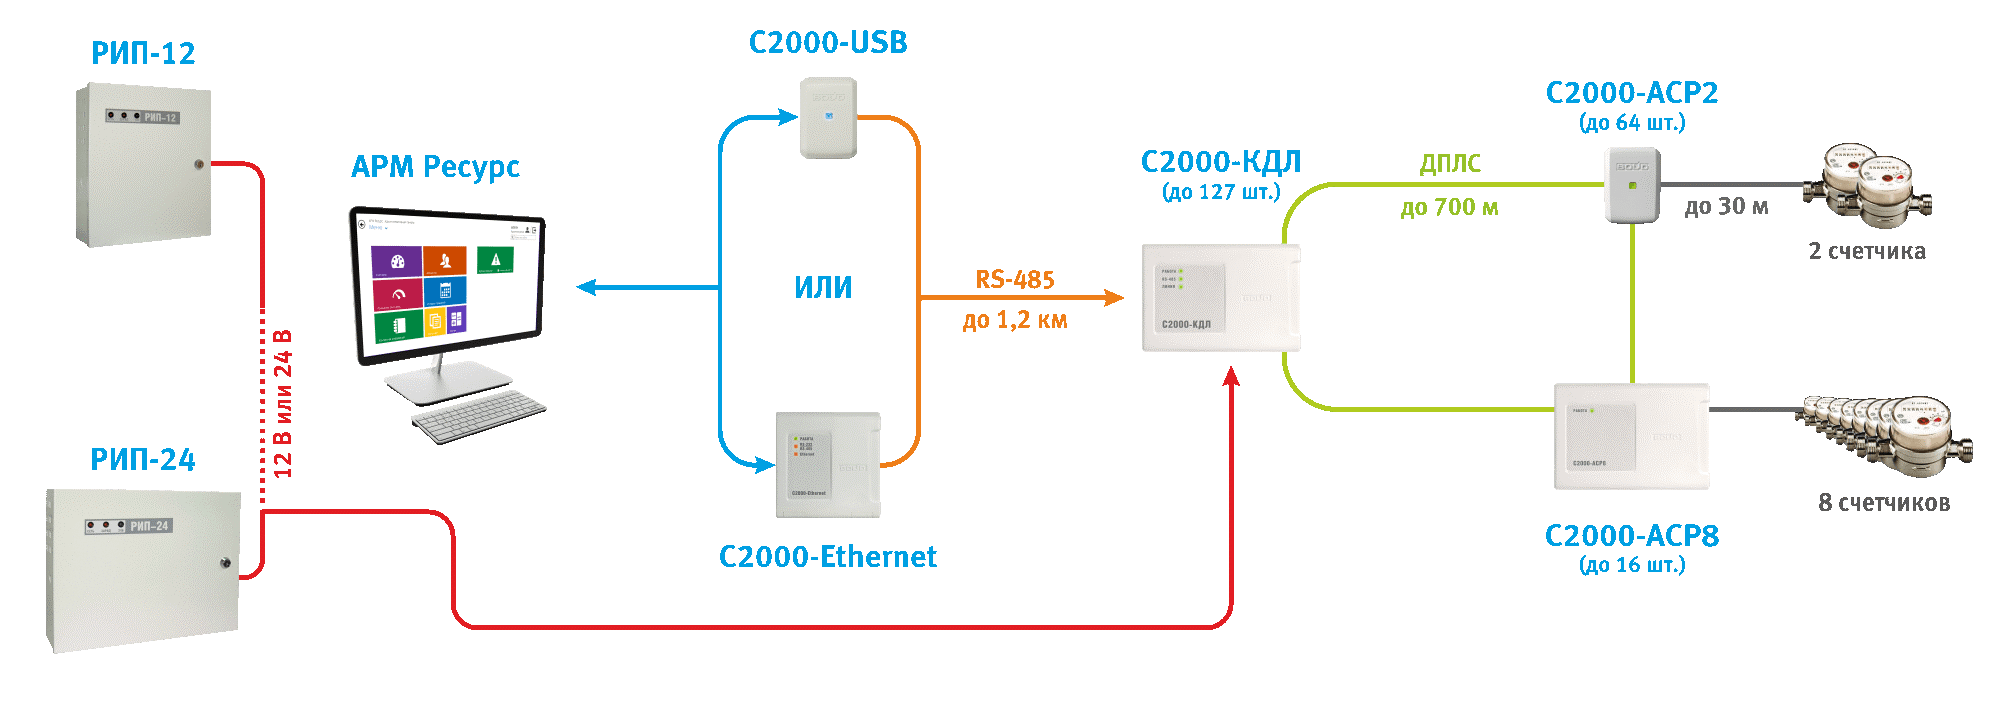
\includegraphics[width=0.7\linewidth]{pics/impuls}
	\caption{Подключение импульсных счётчиков по проводам}
	\label{fig:impuls}
\end{figure}

\begin{figure}[H]
	\centering
	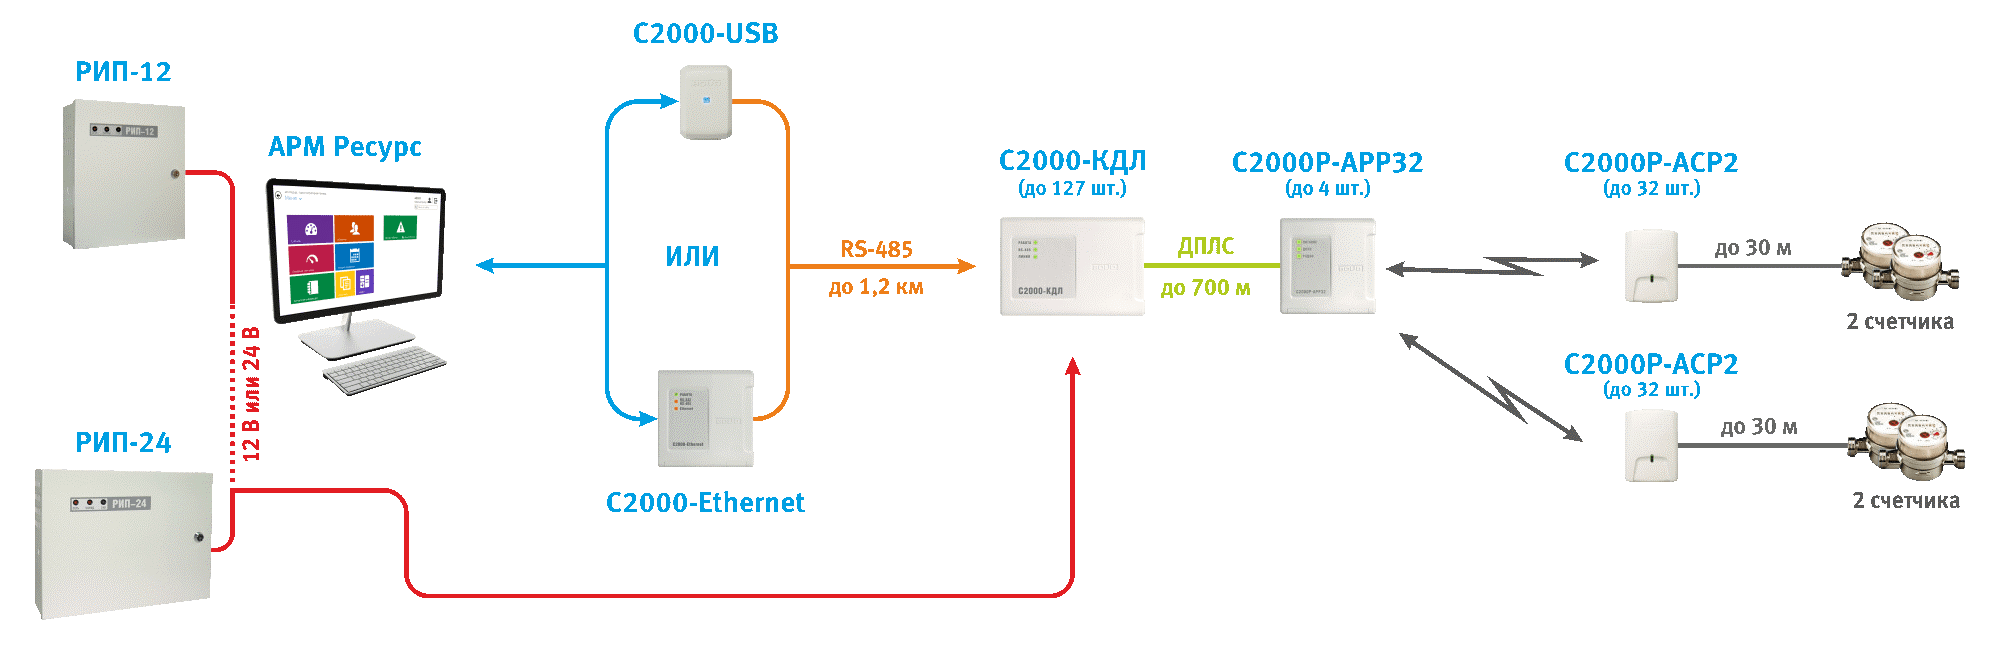
\includegraphics[width=0.7\linewidth]{pics/radio}
	\caption{Подключение импульсных счётчиков по радиоканалу}
	\label{fig:radio}
\end{figure}

\subsubsection{Достоинства и недостатки}

Достоинства:
\begin{itemize}
	\item Система имеет проводные и беспроводные решения;
	\item Наличие личного кабинета; 
	\item Возможность просматривать информацию с помощью web-интерфейса или специальной программы на компьютере;
	\item Наличие резервного питания на устройствах;
\end{itemize}
Недостатки:
\begin{itemize}
	\item Высока стоимость системы в целом из-за большого количества промежуточных устройств и преобразователей;
	\item Из-за линейного подключения устройств система имеет меньшую надежность; \item При выходе из строя одного из устройств не работает вся система;
\end{itemize}

\subsection{Сравнение и оценка}

Объекты сравниваются и оцениваются методом экспертных оценок в таблице~\ref{tab:tab3}. Выбирается ряд параметров, по которым будут оцениваться каждая система. Параметры оценивается по 10-тибальной шкале:
\begin{enumerate}
	\item Стоимость системы (1 – высокая, 10 – низкая) - сравнивается общая стоимость оборудования, технических работ и использования программного обеспечения;
	\item Надёжность системы, работоспособность системы при выходе из строя одного из устройств, а также надёжность передачи и хранения данных (1 – ненадёжная, 10 – очень надёжная);
	\item Безопасность системы (1 – система не безопасна, 10 – высокий уровень) -использование шифрования данных; защита от внешних факторов; защита от взлома; 
	\item Простота ввода системы в эксплуатацию (1 – проблемы с вводом в эксплуатацию, 10 – очень просто) - удобство ввода системы в уже построенные дома. 
	\item Простота замены комплектующих системы (1 – сложно, 10 – очень просто) - настройка нового оборудования; время замены отказавшего устройства на новое.
\end{enumerate}

\begin{table}[H]
	\caption{Сравнение и оценка системы} \label{tab:tab3}
	\centering
	\begin{tabular}{|p{1.4cm}|p{3cm}|p{1cm}|p{3cm}|p{3cm}|p{3cm}|}
		\hline 
		№ & Параметр & Вес & Система "СТРИЖ" & АСКУЭ "Ресурс" & Система "СКАУТ" \\ 
		\hline 
		1 & Стоимость & 0.3 & 2 & 6 & 8 \\ 
		\hline 
		2 & Надёжность & 0.25 & 6 & 5 & 7 \\ 
		\hline 
		3 & Безопасность & 0.1 & 8 & 5 & 5 \\ 
		\hline 
		4 & Простота ввода системы в эксплуатацию   & 0.2 & 9 & 6 & 7 \\ 
		\hline 
		5 & Простота замены комплектующих & 0.15 & 8 & 5 & 8 \\ 
		\hline 
		Сумма & & 1 & 5.9 & 5.7 & 7.05 \\ 
		\hline 
	\end{tabular} 
\end{table}
В результате система «СКАУТ» оказалась более эффективной в сравнении с другими системами. 